\documentclass{article}

\usepackage[margin=1in]{geometry}

% Tables and stopping them from displaying in a different section
\usepackage{booktabs}
\usepackage[section]{placeins}

% for inserting images into the document, setting file path, and allowing rotation of inserted images 
\usepackage{graphicx}
\graphicspath{ {./images/} }
\usepackage{rotating}
\usepackage[table]{xcolor}
% mostly just for putting text in math equations
\usepackage{amsmath}
% for aligning the text to the left
\usepackage[document]{ragged2e}

% for inserting hyperlinks in the document, use \url{url} or \href{url}{text}
\usepackage{hyperref}
\usepackage{siunitx}
\usepackage{caption}
\usepackage{multirow}
\usepackage[export]{adjustbox}

\title{\textbf{Lab 1: Instrumentation}}
\author{Report by: Natalie Tran\\
Performed by: Natalie Tran and Zachary Pouska}
\date{Date performed: 09/12/2022}

\begin{document}
	\maketitle
	\section*{Purpose}
	Learning how to use lab equipment. This includes a Digital Multi-Meter, a Function Generator, a Power Supply, and an Oscilloscope. A range of tests will be performed to get comfortable reading Voltage, Frequency, Period, and Amplitude from the Oscilloscope. \\
	\section*{Results}
	\begin{table}[ht!]
	\begin{center}
	\rowcolors{3}{gray!10}{gray!40}
	\caption{Power Supply vs DMM Voltage}
	\vspace{0.2cm}
	\begin{tabular}{c|c}
		\textbf{Power Supply} & \textbf{ Voltage Measured with}\\
		\textbf{Voltage (V)} & \textbf{the DMM (V)}\\
		\hline
		1.0 & 0.964\\
		2.0 & 2.088\\
		3.0 & 3.262\\
		4.0 & 3.933\\
	\end{tabular} 
\end{center}
\end{table}
\begin{table}[h!]
	\rowcolors{2}{gray!10}{gray!40}
	\caption{Channel Voltage Calibration}
	\begin{center}
	\begin{tabular}{c|c|c|c}
			   & \textbf{Number of Vertical Deflections} & \textbf{Volts/Div Setting} & \textbf{Voltage} \\
			   \hline
		\textbf{Channel 1}  & 1                              & 0.5V              & 0.5V    \\
		\textbf{Channel 2}  & 1                              & 0.5V              & 0.5V    \\
	\end{tabular}
\end{center}
\end{table}
\begin{table}[h!]
	\rowcolors{2}{gray!10}{gray!40}
	\caption{Channel Period Calibration}
	\begin{center}
	\begin{tabular}{c|c|c|c}
			   & \textbf{Number of Vertical Deflections} & \textbf{Sec/Div Setting} & \textbf{Period} \\
			   \hline
		\textbf{Channel 1}  & 2                              & 0.5ms              & 1ms    \\
		\textbf{Channel 2}  & 2                              & 0.5ms              & 1ms    \\
	\end{tabular}
\end{center}
\vspace{2cm}
\end{table}
\begin{table}[ht!]
\begin{center}
	\rowcolors{3}{gray!10}{gray!40}
	\caption{Interpreting Frequency from the Oscilloscope}
	\vspace{0.2cm}
	\begin{tabular}{c|c|c|c}
		\textbf{Frequency from Signal} & \textbf{Number of Horizontal Divisions} & \textbf{Period} & \textbf{Frequency}\\
		\textbf{Generator (Hz)} & \textbf{Peak to Peak} & \textbf{of Signal} & \textbf{(Hz)}\\
		\hline
		50 & 2.4 & 24ms & 41.7\\
		500& 4.8 & 2.4ms & 417\\
		800& 6.7 & 1.3ms & 746\\
		2500&7.4 & 0.74ms& 1350\\
		5000&4.7 & 235$\mu$s&4260\\
		6500&8.4&168$\mu$s&5950\\
		8000&6.9&138$\mu$s&7250\\

	\end{tabular}
\end{center}
\end{table}
\vspace{0.8cm}
	    \begin{minipage}[t]{0.5\textwidth}
		  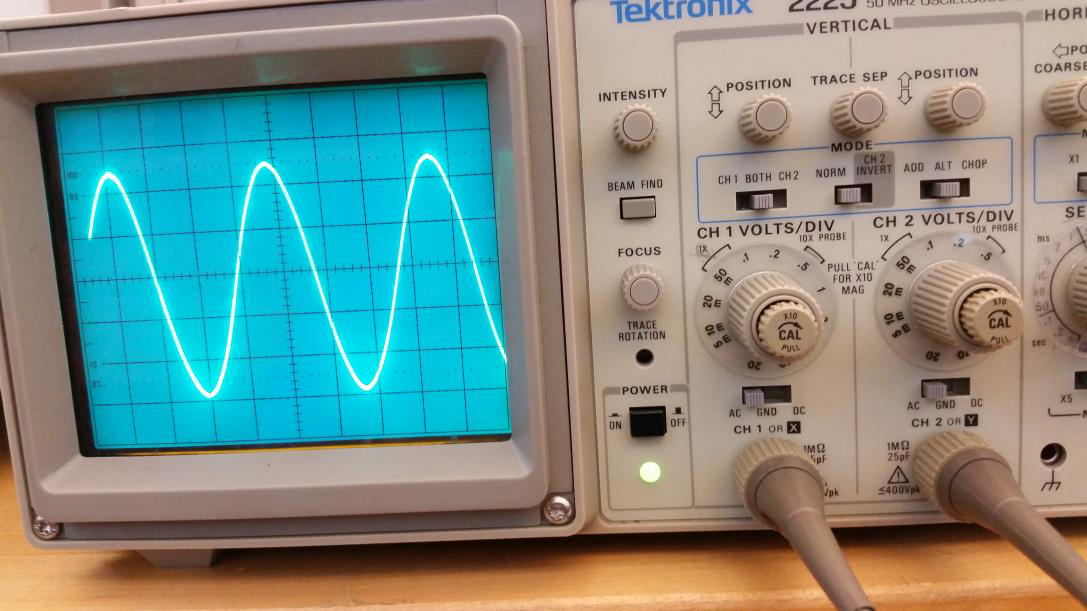
\includegraphics[width=0.99\linewidth, frame]{example1}\\
			 Figure 1: Ocilloscope Calibrated to 0.5 Volt/Div and 0.5 ms/Div
	     \end{minipage}
	      \hfill
	     \begin{minipage}[b]{0.4\textwidth}
		 \begin{center}
		 \begin{tabular}{|l|l|}
			 \hline
			 Voltage$_{pp}$ & 2.75V \\
			 Voltage$_{p}$ & 1.375V \\
			 Voltage$_{rms}$ & 0.972V \\
			 Period & 1.9ms \\
			 Frequency & 526.0hz \\
			 \hline
			 \end{tabular}	
		 \end{center}
		 \vspace{0.5cm}
		 \begin{center}
			Analyzed Table for Fig.1
		 \end{center}
		 \end{minipage}
		 \vspace{0.8cm}
		 \begin{table}[h]
			 \begin{center}
			\rowcolors{2}{gray!10}{gray!40}
			\caption{Analyzed V$_{rms}$ vs DMM V$_{rms}$}
		\begin{tabular}{c|c|c|c|c|c}
			\textbf{Trial} & \textbf{V$_{pp}$} &\textbf{ V$_{p}$} & \textbf{Calculated V$_{rms}$} &\textbf{ DMM V$_{rms}$} &\textbf{Percent Difference}\\
			\hline
			1* & 1.0 &N\slash A &N\slash A &N\slash A &N\slash A \\
			2* & 1.5 &N\slash A &N\slash A &N\slash A &N\slash A \\
			3 & 2.0 &1 &0.707 &0.621 &12.9\% \\
			4 & 3.0 &1.5 &1.06 &0.995 &6.32\% \\
			5 & 4.0 &2 &1.414 &1.348 &5.48\% \\
			6 & 6.0 &3 &2.121 &2.000 &5.87\%\\
			7 & 8.0 &4 &2.828 &2.666 &5.90\%\\


		\end{tabular}\\
	\textit{*Trials 1 and 2 were not performed due to the frequency generator's inability to achieve a low voltage.}
	\end{center}
	\end{table}
	Voltage$_{rms}$ is calculated using the equation:
	\[
		V_{rms} = \frac{1}{\sqrt{2}} * V_{p}
	\]
	\begin{table}[ht]
		\begin{center}
			\captionsetup{justification=centering,margin=2cm}
		\caption{Calculating Voltage$_{pp}$ and Frequency of Waves on the New and Old Oscilloscope Generated by an External and Internal Frequency Generator.}
			\rowcolors{4}{gray!10}{gray!40}
		\begin{tabular}{c|c|c|c|c|c|c}
		   Frequency	& \multicolumn{2}{c|}{Signal}& \multicolumn{2}{c|}{Old}& \multicolumn{2}{c}{New}\\
			\cline{2-7}
			Generator&Type of Wave &Frequency (Hz)&V$_{pp}$&Frequency (Hz)&V$_{pp}$&Frequency (Hz)\\
			\hline
			\cellcolor{white} &sine &  1000 & 4 & 1000 & 3.8 & 1020 \\
			\cellcolor{white} &sine &2000&3.8&2083&3.8&2130\\
			\cellcolor{white}\multirow{-3}{*}{External}&sine&5000&3.8&5333&3.6&5.26\\
			\hline
			\cellcolor{white} &square&1000&8&1000&8.5&1000\\
			\cellcolor{white}&square&2000&8&2000&8.5&2000\\
			\cellcolor{white} \multirow{-3}{*}{Oscilloscope}&square&3000&8&3130&8.5&3000\\
		\end{tabular}
	\end{center}
	\end{table}
	\section*{Questions}
	\begin{enumerate}
	\item \textbf{What is the purpose of an oscilloscope?}\\
		Graphically displaying changes in Voltage.
		 \item \textbf{What is the difference among peak-to-peak voltage, peak voltage, and rms voltage?}\\
			 Voltage$_{pp}$ is measured to be double the amplitude, or from the highest point to the lowest point. Voltage$_{p}$ is the half of Voltage$_{pp}$, or the amplitude measured from the highest or lowest point to zero. Voltage$_{rms}$ stands for 'Root Mean Square' of the voltage, giving the mean voltage over half a period. 
	\item \textbf{What electrical variables can be measured with the digital multimeter?}\\
	Amperes (A), Voltage (V), and Ohms (\si{\ohm}) can be measured from a digital multimeter.
	\end{enumerate}
	\textbf{Using the oscilloscope, set up a sine function coming from the function generator and calculate the voltage peak-to-peak, voltage peak, voltage rms, and the period of the signal.\\
	Case 1: 2 Volt/Div and 0.2 ms/Div\\
Case 2: 5 Volt/Div and 50$\mu$s/Div\\}
	\begin{table}[h]
		\begin{center}
		\rowcolors{2}{gray!10}{gray!40}
		\begin{tabular}{l|c|c}
			& \textbf{Case 1} & \textbf{Case 2}\\
			\hline
			Voltage$_{pp}$ (V)& 8&20\\
			Voltage$_{p}$ (V)&4&10\\
			Period&0.84ms&210$\mu$s\\
			Frequency (Hz)&1190&4762\\
		\end{tabular}
		\end{center}
	\end{table}
		\section*{Conclusion}
Overall, the main purpose of this lab was achieved, although there was a lack in usage of the newer oscilloscope with the built-in function generator. Reading the voltage and period on the older oscilloscope became comfortable, along with calculating voltage$_{rms}$ and frequency. Though, there were many challenges along the way. It was difficult to accurately read the oscilloscope due to the impercision of the graph the generated frequencies were displayed on. The frequency generator was also tough to calibrate to a specific frequency due to an inaccurate calibration knob. Some equipment were also unreliable, producing incorrect frequencies or voltages. An abundance of human error is also present in the results, as many readings were eyeballed, and given the best estimation possible. This resulted in mismatches in the calculated frequency and voltage. 
	
\end{document}
